\section{问题四模型的建立与求解}

问题四把问题三的固定电价改为\textbf{实时波动的电价}（附件 4），要求在波动电价下重新计算问题二与问题三：问题 4-2 每天 0:00 只制定一次计划购电量、日内不改；问题 4-3 每天 0:00 制定原计划，6:00、12:00、18:00 根据新光伏预报与最新价格信息调整尚未执行的购电量。问题四相对问题三的实质新增在于\textbf{电价的不确定性}：查阅相关资料可知，电价本质上反映电力供需关系，因而同时受日内负荷波动、工作日与周末用电结构差异、季节性负荷等多重时间尺度影响，故不能把固定价数组简单替换成均值，而必须显式刻画电价的多尺度规律并将其不确定性纳入随机规划。除电价外，其余结构（单 W 能量平衡、SOC 递推、调整结算、跨日终端价值 $\theta$、情景 MPC、报童下界、同季节条件化）与问题三完全一致，本文不再重复。

\subsection{数据预处理与探索性分析}

与问题三相同，附件 4 的波动电价数据经核对\textbf{无缺失值、无异常值、无量纲不一致}，数据完整可用，无需专门预处理。其电价范围为 $0.0076$--$1.7936$ 元/kWh，全年每日峰谷价差中位数约 $1.056$ 元/kWh，说明价格波动幅度可观、峰谷价差足以显著改变储能充放电的先后顺序。

考虑到电价受多尺度因素共同驱动，我们对电价作三层分解。观察电价的日内曲线可以发现，电价呈现与负荷类似的\textbf{峰谷形态}：白天用电高峰对应电价高位、凌晨低谷对应低位，这一“昼夜”规律源于电力供需的日内周期波动，也意味着储能存在明显的日内套利空间。进一步观察发现，电价还表现出明显的\textbf{周周期}：上周同一时刻的价格是本周价格的最强预测线索（滚动 WAPE 约 6.22\%），且工作日与周末价格水平存在系统性差异，符合工商业负荷集中于工作日的常识。电价水平还随季节缓慢漂移，冬季与夏季因取暖、制冷负荷而整体偏高。综合以上三个尺度，电价可分解为“季节基线 + 周内偏移 + 日内峰谷”的叠加结构，这正是电价预测模型的设计依据。

\subsection{模型建立}

\subsubsection{符号设定}

沿用问题三全部符号，新增电价相关符号：$P_{d,t}$ 为实际波动电价，$\widehat P_{d,t}$ 为电价预测，$P^\omega_{d,t}$ 为情景电价，$m^p_{d,t}$ 为周同期基线，$\bar P^{\mathrm{seas}}_{d,t}$ 为季节基线，$\gamma^p_{d,t}$ 为日内时段效应，$\delta^p_{d,r}$ 为水平修正，$\varepsilon^p_{j,t}$ 为电价预测残差。

\subsubsection{电价三尺度因果预测}

基于探索性分析的三尺度结构，电价预测依次叠加四部分。季节基线取同季节历史日均价曲线 $\bar P^{\mathrm{seas}}_{d,t}$；周同期基线取上周同一时刻价格 $m^p_{d,t}=P_{d-7,t}$（冷启动用季节基线）；日内时段效应 $\gamma^p_{d,t}$ 从同星期历史日的周残差中估计并经零和化，只描述昼夜中稳定的峰谷偏移；水平修正 $\delta^p_{d,r}$ 用最近至多 36 个已实现价格估计当天整体水平并截断。最终电价预测为
\begin{equation}
\widehat P_{d,t}=\max\Big\{\varepsilon_p,\ m^p_{d,t}+\gamma^p_{d,t}+\delta^p_{d,r}\Big\}.\label{eq:price4}
\end{equation}
三尺度对应关系清晰：昼夜由 $m^p$ 的日内形状与 $\gamma^p$ 的日内峰谷共同描述，周内由 $m^p=P_{d-7,t}$ 的周周期描述，季节由 $\bar P^{\mathrm{seas}}$ 与 $\delta^p$ 描述。

\subsubsection{负载—光伏—电价联合情景}

对历史日 $j<d$ 因果重放三类残差 $\varepsilon^L,\varepsilon^R,\varepsilon^p$，再从与 $d$ 同季节的历史日中抽取同一历史日的整段残差构造三元情景
\begin{equation}
L^\omega=\max\{0,\widehat L+\varepsilon^L\},\quad R^\omega=\max\{0,\widehat R+\varepsilon^R\},\quad P^\omega=\max\{\varepsilon_p,\widehat P+\varepsilon^p\}.\label{eq:scenario4}
\end{equation}
三类残差必须来自同一历史日整段块，以保留“高负荷、低光伏、高电价”之间的同期相关性。

\subsubsection{优化模型（价格情景化）}

问题四的物理约束与问题三完全相同，仅把目标与结算中的固定价换成情景价（优化）或实际价（结算）。问题 4-3 第 $k$ 次更新的目标为
\begin{equation}
\min\ \sum_{\omega}\pi_\omega\Big[\sum_{t\in\mathcal R_k}\big(P^\omega_{d,t}G^{(k)}_{d,t}+0.5P^\omega_{d,t}A^{(k)}_{d,t}+5P^\omega_{d,t}E^\omega_{d,t}\big)+\theta^\omega\Big].\label{eq:obj4}
\end{equation}
执行层情景 MPC 的目标相应为 $\min\sum_\omega\pi_\omega[\sum_{t=r}^{144}5P^\omega_{d,t}E^\omega_{d,t}+\theta^\omega]$，当前区间电价用实际价、未来电价用情景价。官方结算用真实价格 $P_{d,t}$ 复算。

\subsection{模型求解}

问题四沿用问题三的滚动求解流程、Step 式步骤与并行结构，仅在预测层增加电价三尺度预测、在情景层增加电价一维；各子问题仍为连续线性规划，统一采用 SciPy 的 \texttt{scipy.optimize.linprog}（HiGHS 方法）求解。电价情景只是在情景矩阵中多一维 $P^\omega$，不改变 LP 规模，故每策略计算成本与问题三同级。四组配置（C2、C3、PI2、PI3）进程级并行。

\subsection{结果分析}

\subsubsection{模型验证}

能量平衡、SOC 递推、费用复算三类残差均通过（分别约 $4.5\times10^{-13}$、$9\times10^{-13}$、$3.7\times10^{-9}$，无违规），说明波动电价下的求解同样稳定。

问题四的官方结算费用与\textbf{价格信息价值}见表~\ref{tab:info4}。价格信息价值定义为有限年度费用差 $\widehat{\Delta C}^p=C_{\text{因果}}-C_{\text{完美价格}}$，即“提前知道当天完整电价”相对“因果预测电价”能节省的费用。

\begin{table}[htbp]
\centering
\caption{问题四官方结算费用与价格信息价值（万元）}
\label{tab:info4}
\begin{tabular}{ccccc}
\toprule
配置 & C2（4-2 因果） & C3（4-3 因果） & 信息价值 4-2 & 信息价值 4-3 \\
\midrule
下界 0.8、MPC5 & 1862.8 & 1939.9 & $-0.7$ & $-0.03$ \\
无下界、MPC5 & 1710.5 & 1628.8 & $+4.4$ & $+14.1$ \\
无下界、MPC50 & 1518.5 & 1533.6 & $+14.2$ & $+16.2$ \\
\bottomrule
\end{tabular}
\end{table}

观察表~\ref{tab:info4} 可以发现：在报童下界 q=0.8 时价格信息价值几乎为零（甚至略负），关掉下界后转为正值，且随 MPC 情景数增加而进一步增大。这一规律具有明确的经济含义——计划越保守，越不需要“精确价格”这一额外信息；只有当计划真正依赖价格预测时，完美价格信息才能转化为实际经济收益。可见价格信息的价值并非固定，而是由决策框架的对冲程度内生决定。

除价格信息价值外，波动电价对微网的运行形态也产生了可观测的影响。图~\ref{fig:q4_monthly} 给出固定电价（问题三）与波动电价（问题四 4-2、4-3）下月度购电费用与紧急购电需求的对比。

\begin{figure}[htbp]
\centering
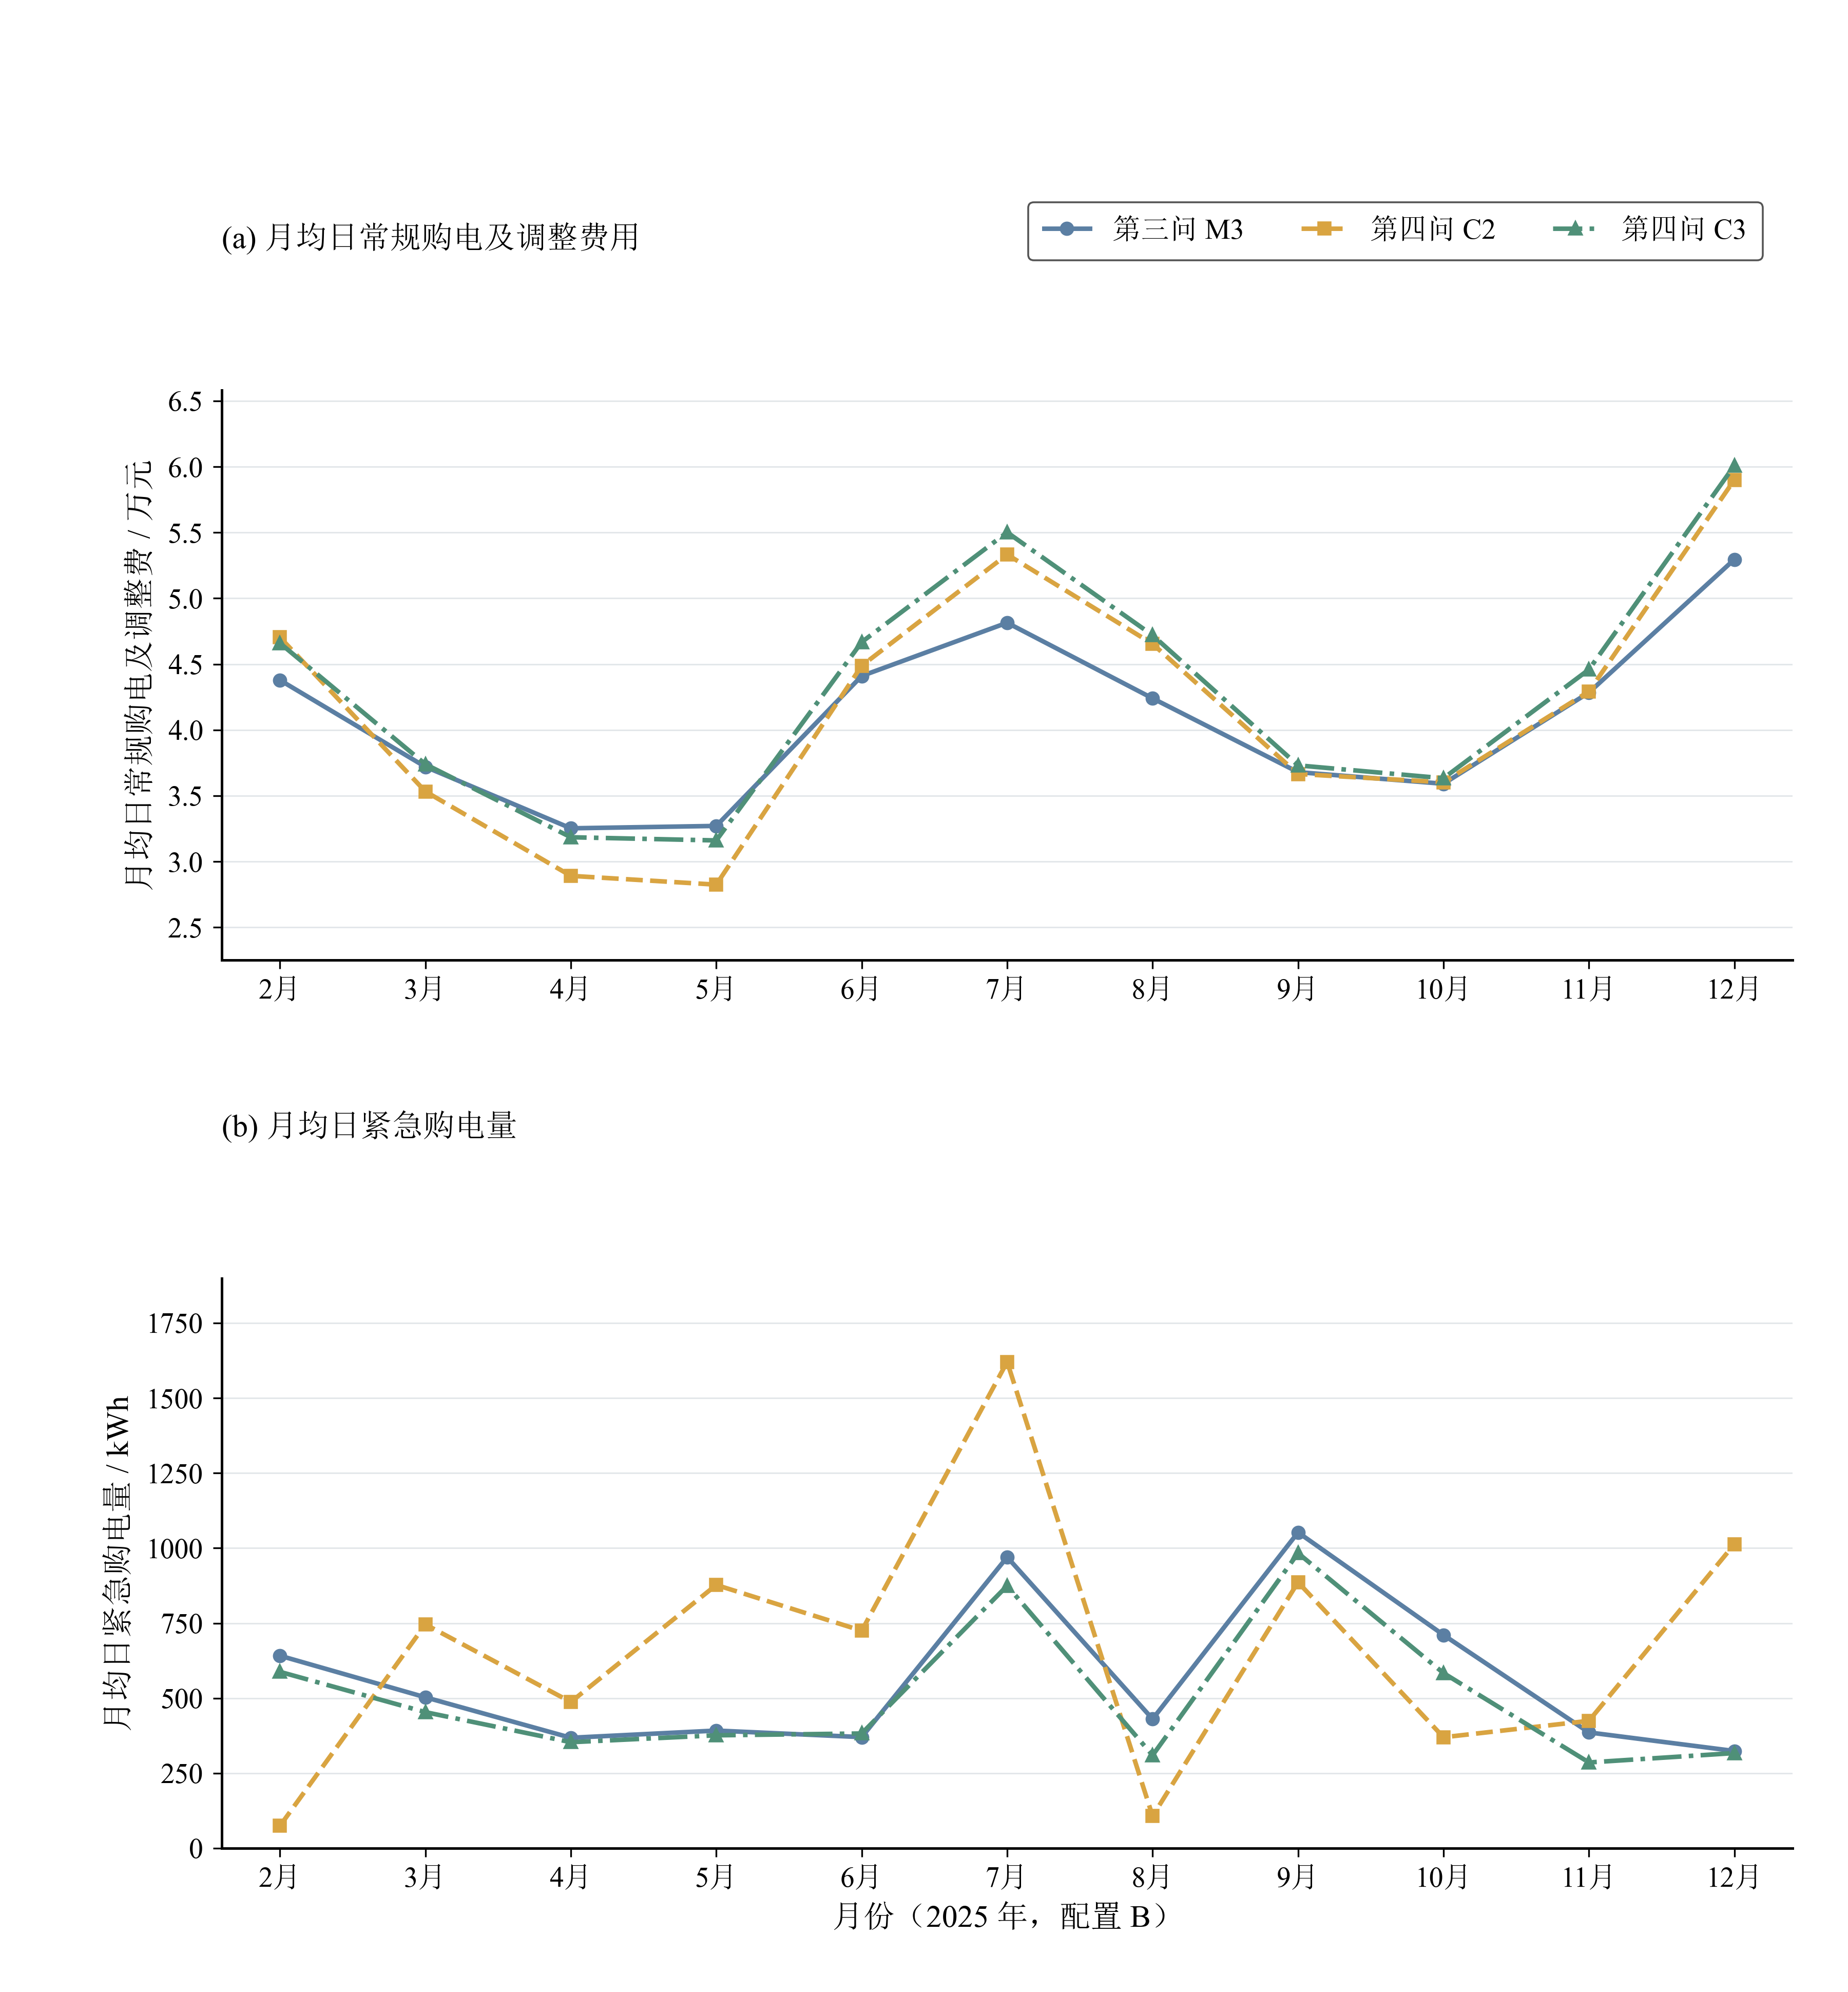
\includegraphics[width=0.55\textwidth]{figures/05_monthly_operation.png}
\caption{固定电价与波动电价下月度购电费用与紧急购电需求}
\label{fig:q4_monthly}
\end{figure}

观察图~\ref{fig:q4_monthly} 可以发现，两类电价下的购电费用与紧急购电需求都保持相似的季节性轮廓——冬季负荷高、光伏低时抬升，但波动电价使各月的购电费用出现重新排序：价格高企的月份购电费用相对上升，价格低谷的月份则相对下降，说明电价的多尺度波动通过改变储能套利与计划购电的时机，重塑了全年费用的月度分布。图~\ref{fig:q4_storage} 进一步从日内与日末两个维度刻画储能运行的变化。

\begin{figure}[htbp]
\centering
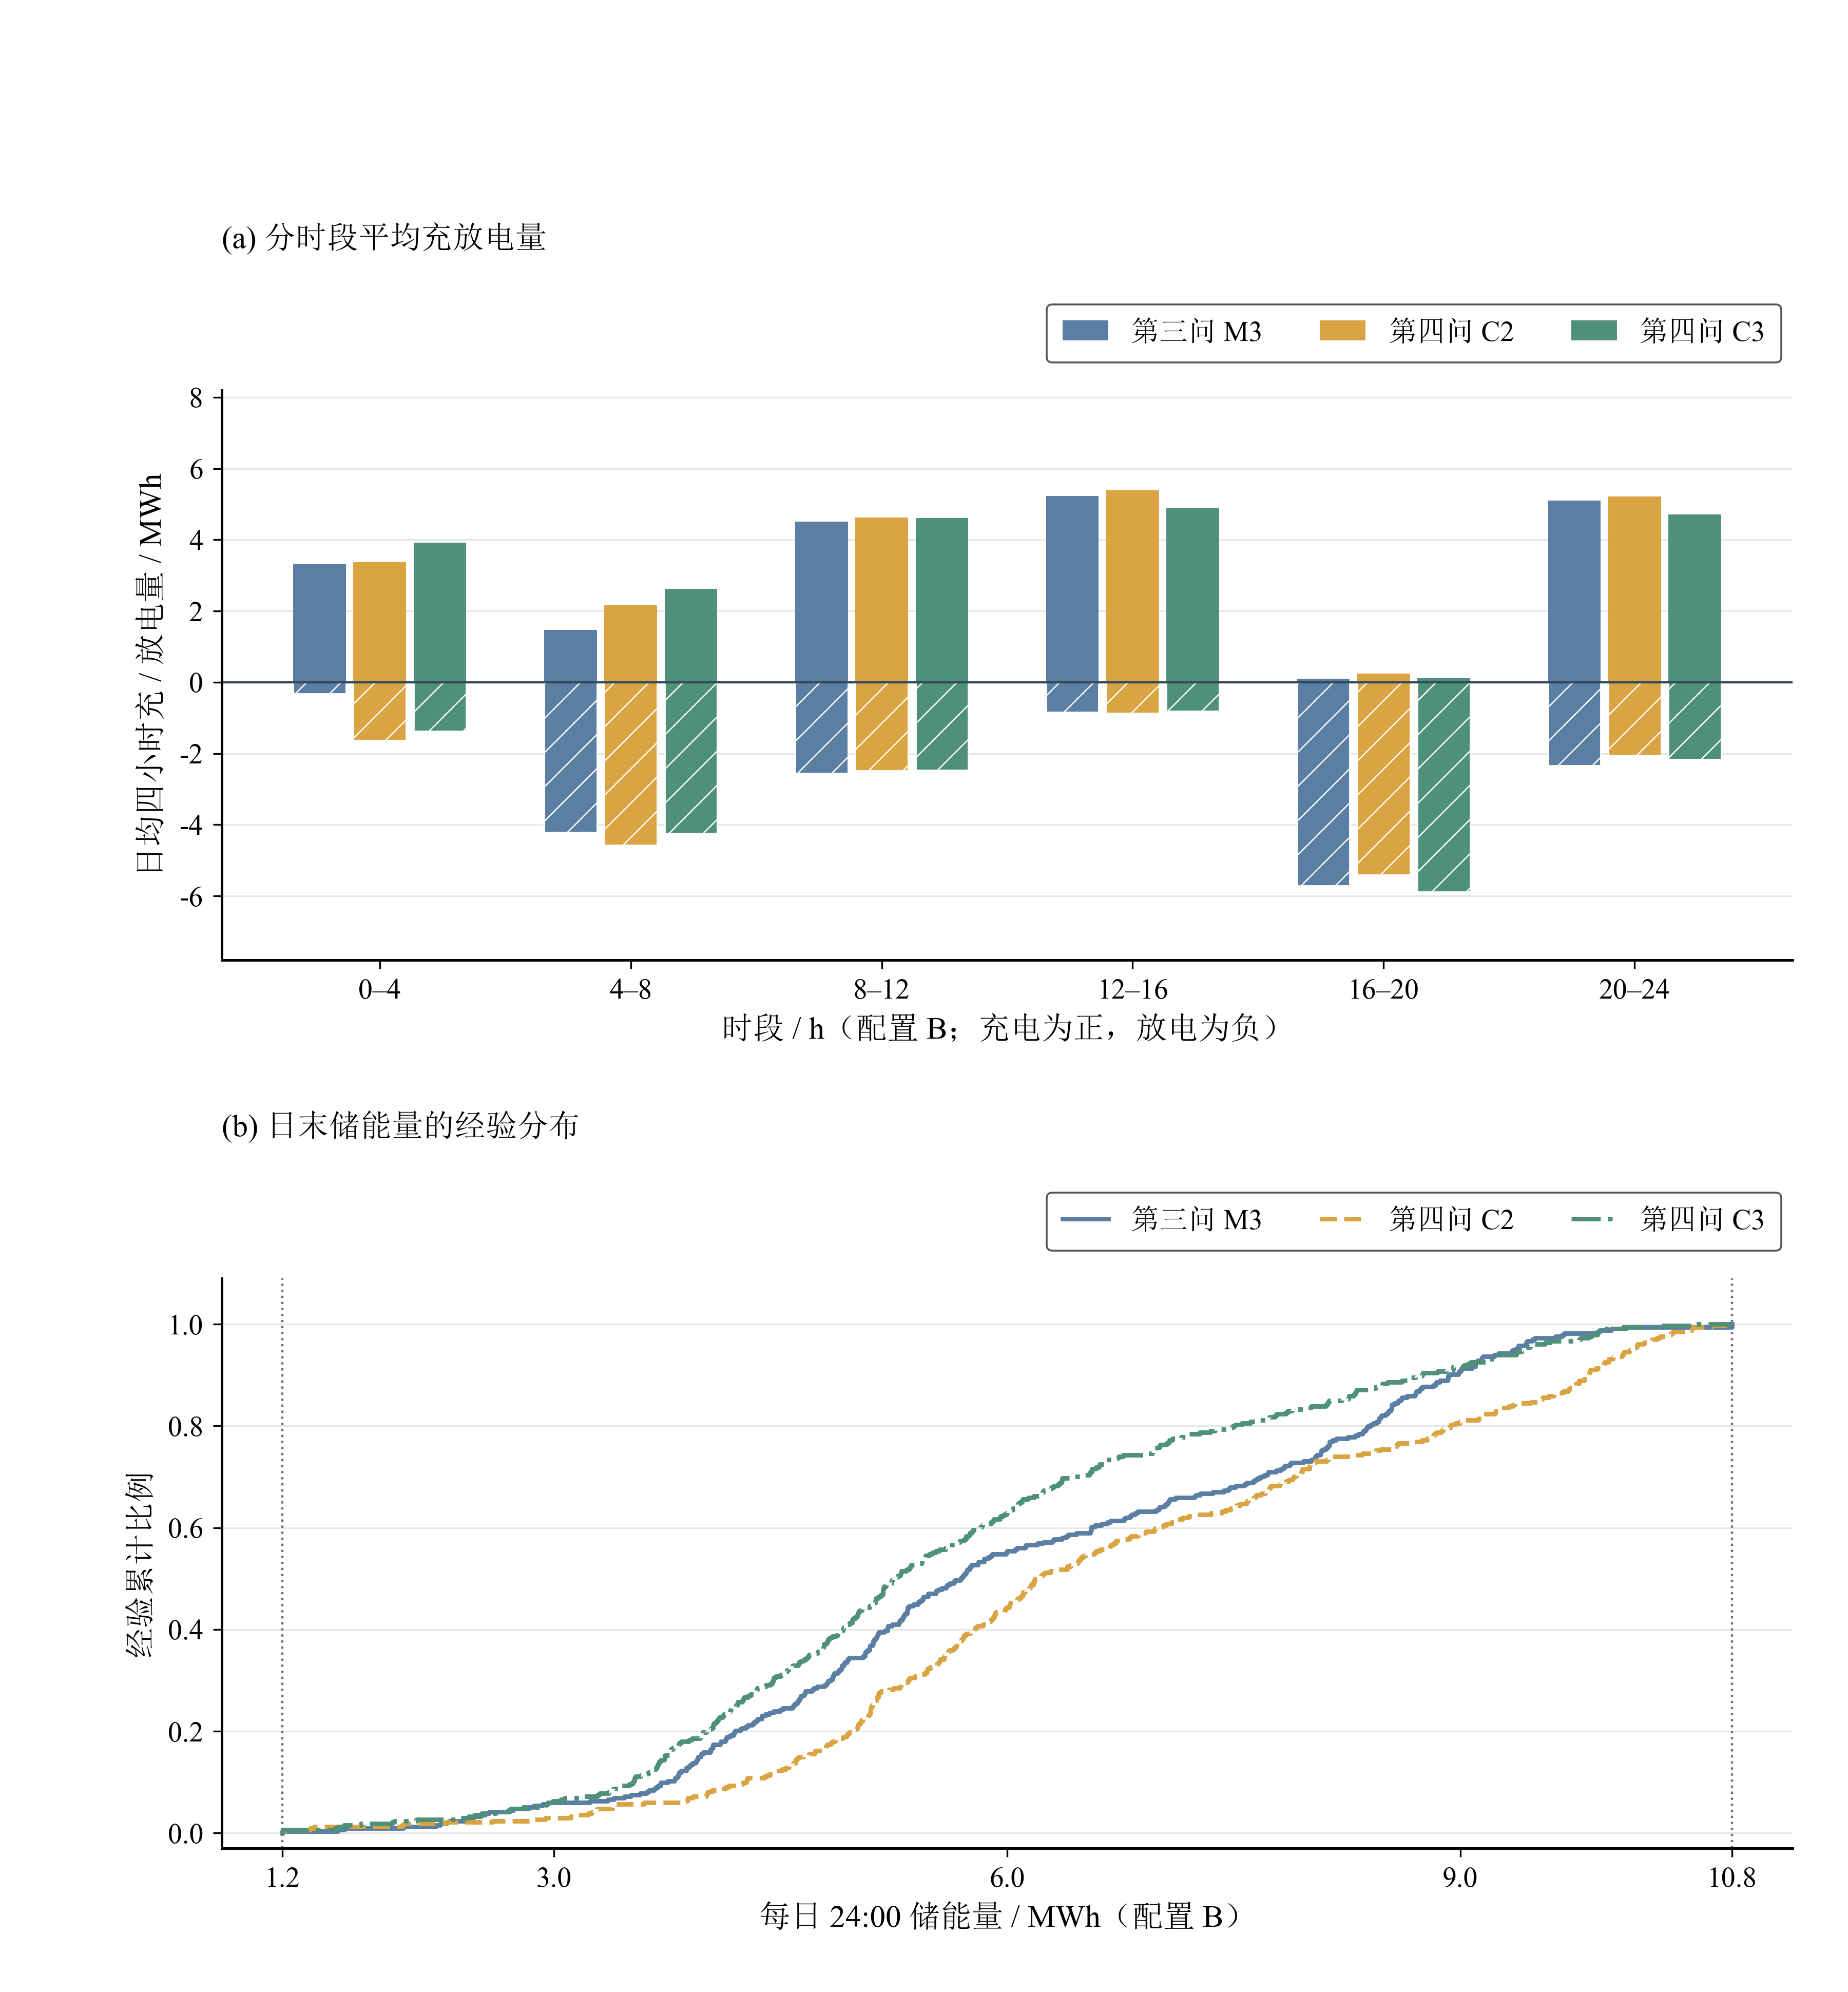
\includegraphics[width=0.55\textwidth]{figures/06_storage_operation.png}
\caption{固定电价与波动电价下储能日内充放电与隔夜储能}
\label{fig:q4_storage}
\end{figure}

观察图~\ref{fig:q4_storage} 可以发现，储能依然保持“充电与放电交替”的日内套利形态，但波动电价下充放电的时段位置更贴近电价峰谷而非单纯负荷峰谷；同时日末储能量仍稳定维持在安全区间中高位，说明终端价值 $\theta$ 在波动电价下同样维持了隔夜缓冲。可见，价格信号与负荷/光伏信号共同作用于储能，储能既削峰填谷又套利，但并未因价格波动而破坏跨日保电的稳健性。

\subsubsection{价格信息口径的敏感性分析}

本文区分“因果价格预测”与“完美价格信息（PI-DA，每天 0:00 已知当天全价）”两种口径：前者是实际可执行的方案，后者是信息基准。如模型验证所示，两者费用差随计划保守程度递减，说明在本文的滚动随机规划框架下价格信息的边际价值有限；但这一结论依赖报童下界与情景 MPC 的对冲强度，不能外推到更简单的确定性模型。

\subsubsection{小结}

问题四把问题三的固定价换成波动价：先用“季节基线 + 周同期基线 + 日内时段效应 + 水平修正”显式刻画电价的昼夜、周内、季节三尺度规律，再与负载、光伏一起抽成同一历史日的三元联合残差情景，喂给与问题三完全相同的两阶段随机规划 + 情景 MPC + 报童下界 + 终端价值框架，最终用真实价格结算。价格信息价值实验表明其经济价值随计划保守程度递减，这既印证了模型对冲机制的合理性，也为“是否需要更精确的价格预测”提供了可量化的判断依据。
